Attribution methods assign substantially different shares to the same feature groups.
Figure~\ref{fig:attribution_method_comparison} compares the methods on the common eligible POIs in the fixed sample of 1,024 locations.
In December, the mean history share is \(58.1\%\) under Gradient \(\times\) Input and \(74.6\%\) and \(87.2\%\) under the two IG references.
The parent share falls from \(18.2\%\) to \(2.1\%\) and \(1.1\%\), respectively.
January reproduces this pattern, so attribution magnitudes depend strongly on the method and reference input even with the fitted predictor held fixed.

\begin{figure}[!htbp]
\centering
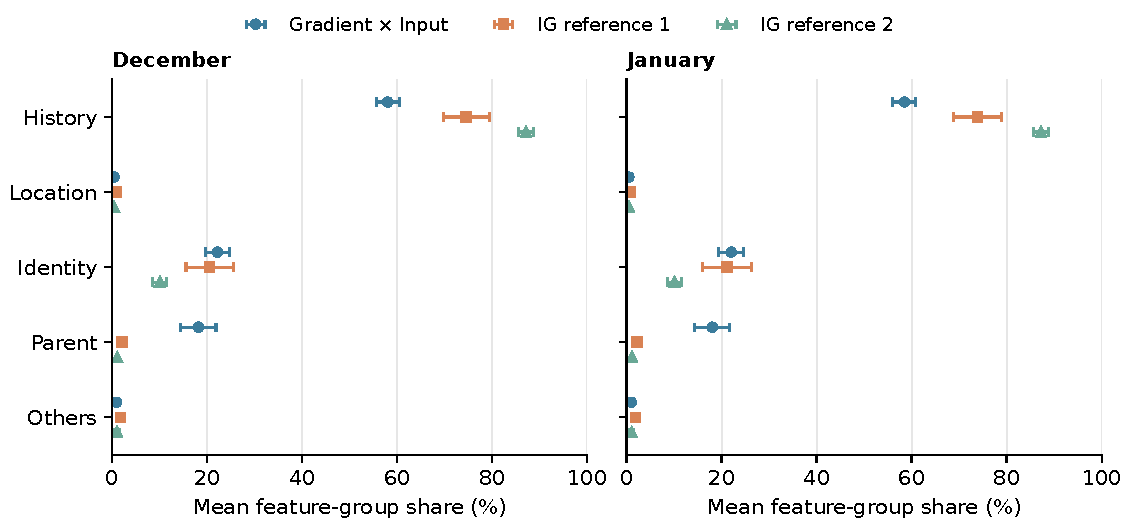
\includegraphics[scale=0.65]{art/attribution_method_comparison.pdf}
\caption{Mean feature-group shares on the common eligible POIs in the 1,024-POI sample at \(T=14\), \(H=7\). Points and bars show means and standard deviations across the five fitted seeds. Each method uses the same eight origins and seven leads within a month.}
\label{fig:attribution_method_comparison}
\end{figure}

The resulting regime assignments also vary across fitted seeds and attribution methods, as Table~\ref{tab:attribution_stability} shows.
December agreement between Gradient \(\times\) Input and the two IG references is only \(21.3\%\) and \(22.9\%\), and mean agreement across the ten fitted-seed pairs is \(50.4\%\).
January gives similar method agreement of \(21.2\%\) and \(23.1\%\).
Holding the fitted models fixed, the December and January consensus assignments agree for \(74.2\%\) of the 9,817 POIs assigned in both months.
Thus, changing the attribution method alters regime membership more than moving these fitted models to the following month.
The category patterns and map in Appendix~\ref{app:descriptive_attribution} describe the Gradient \(\times\) Input representation.
All 1,895 POIs assigned to the parent-driven consensus regime lack a recorded parent place, so their attribution concerns the learned missing-parent category.
We therefore examine recorded parent places separately in Section~\ref{subsubsec:parent_results} and assess feature utility through retraining.

\begin{table}[!htbp]
\centering
\begingroup
\singlespacing
\fontsize{9pt}{10.5pt}\selectfont
\setlength{\tabcolsep}{4pt}
\renewcommand{\arraystretch}{1.08}
\caption{Attribution stability. Method comparisons use the same 1,024 sampled POIs and forecast events; regime agreement reports the mean and SD across five seeds. The last row in each period averages the ten seed-pair comparisons over all eligible POIs. Remaining columns are mean Spearman rank correlations for feature-group shares. Zero-attribution profiles are excluded.}
\label{tab:attribution_stability}
\begin{adjustbox}{max width=\linewidth}
\begin{tabular}{llrrrrrr}
\toprule
Period & Comparison & Agreement (\%) & History & Location & Identity & Parent & Others \\
\midrule
December & Gradient $\times$ Input / IG 1 & $21.3\pm 7.7$ & -0.06 & 0.51 & -0.07 & -0.30 & 0.05 \\
December & Gradient $\times$ Input / IG 2 & $22.9\pm 7.1$ & -0.12 & 0.90 & -0.20 & -0.30 & 0.06 \\
December & IG 1 / IG 2 & $24.8\pm 2.8$ & 0.08 & 0.61 & 0.03 & 1.00 & -0.77 \\
December & Different fitted seeds & 50.4 & 0.77 & 0.86 & 0.69 & 0.63 & 0.59 \\
January & Gradient $\times$ Input / IG 1 & $21.2\pm 8.8$ & -0.04 & 0.53 & -0.06 & -0.30 & 0.04 \\
January & Gradient $\times$ Input / IG 2 & $23.1\pm 7.3$ & -0.16 & 0.90 & -0.25 & -0.29 & 0.07 \\
January & IG 1 / IG 2 & $25.0\pm 3.2$ & 0.09 & 0.63 & 0.03 & 1.00 & -0.78 \\
January & Different fitted seeds & 50.2 & 0.77 & 0.86 & 0.68 & 0.61 & 0.60 \\
\bottomrule
\end{tabular}
\end{adjustbox}
\endgroup
\end{table}

